\clearpage
\VerdierPhysicalPageAnchor{0094}%
\begingroup
\setlength{\abovedisplayskip}{4pt plus 2pt minus 2pt}%
\setlength{\belowdisplayskip}{4pt plus 2pt minus 2pt}%
\VerdierSemanticAnchor{ch1-3-2-12}
\noindent\textbf{命題 3.2.12.}\quad
\VerdierSemanticAnchor{ch1-3-2-12-a}
a) 射 $c(I)\colon c(g)\longrightarrow c(c(D))$ はホモトピー同値である。

\VerdierSemanticAnchor{ch1-3-2-12-b}
b) 図式

\VerdierSemanticAnchor{ch1-3-2-12-eq1}
\begin{equation}
  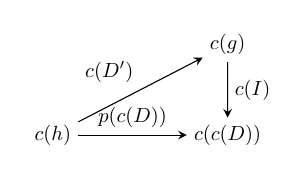
\begin{tikzpicture}[>=stealth,baseline=(current bounding box.center),scale=0.74,
    every node/.style={transform shape}]
    \node (Ch) at (0,0) {$c(h)$};
    \node (Cg) at (3.0,1.55) {$c(g)$};
    \node (CcD) at (3.0,0) {$c(c(D))$};
    \draw[->] (Ch) -- node[above left] {$c(D')$} (Cg);
    \draw[->] (Cg) -- node[right] {$c(I)$} (CcD);
    \draw[->] (Ch) -- node[above] {$p(c(D))$} (CcD);
  \end{tikzpicture}
  \tag{3.2.12.1}
\end{equation}
はホモトピーを除いて可換である。

\VerdierSemanticAnchor{ch1-3-2-12-c}
c) 図式

\VerdierSemanticAnchor{ch1-3-2-12-eq2}
\begin{equation}
  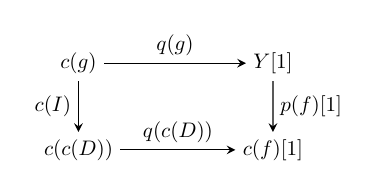
\begin{tikzpicture}[>=stealth,baseline=(current bounding box.center),scale=0.76,
    every node/.style={transform shape}]
    \node (Cg) at (0,1.45) {$c(g)$};
    \node (Y) at (3.25,1.45) {$Y[1]$};
    \node (CcD) at (0,0) {$c(c(D))$};
    \node (Cf) at (3.25,0) {$c(f)[1]$};
    \draw[->] (Cg) -- node[above] {$q(g)$} (Y);
    \draw[->] (Cg) -- node[left] {$c(I)$} (CcD);
    \draw[->] (Y) -- node[right] {$p(f)[1]$} (Cf);
    \draw[->] (CcD) -- node[above] {$q(c(D))$} (Cf);
  \end{tikzpicture}
  \tag{3.2.12.2}
\end{equation}
は可換である。

\VerdierSemanticAnchor{ch1-3-2-12-component-calculation}
実際、直接計算すれば、射 $c(I)$ の第 $i$ 成分は

\VerdierSemanticAnchor{ch1-3-2-12-eq3}
\begin{equation}
  c(I)^i=
  \begin{pmatrix}
    \operatorname{id}&0\\
    0&0\\
    0&\operatorname{id}\\
    0&0
  \end{pmatrix}
  \colon Z^i\oplus Y^{i+1}\longrightarrow
  Z^i\oplus X^{i+1}\oplus Y^{i+1}\oplus X^{i+2}.
  \tag{3.2.12.3}
\end{equation}
であることが分かる。

\VerdierSemanticAnchor{ch1-3-2-12-inverse}
射 $u\colon c(c(D))\longrightarrow c(g)$ の成分を

\VerdierSemanticAnchor{ch1-3-2-12-eq4}
\begin{equation}
  u^i=
  \begin{pmatrix}
    \operatorname{id}&0&0&0\\
    0&f^{i+1}&\operatorname{id}&0
  \end{pmatrix}
  \colon Z^i\oplus X^{i+1}\oplus Y^{i+1}\oplus X^{i+2}
  \longrightarrow Z^i\oplus Y^{i+1}
  \tag{3.2.12.4}
\end{equation}
と定めると、これはホモトピーを除いて $c(I)$ の逆であり、第一の主張が
証明される。第二の主張を証明するには、図式

\VerdierSemanticAnchor{ch1-3-2-12-eq5}
\begin{equation}
  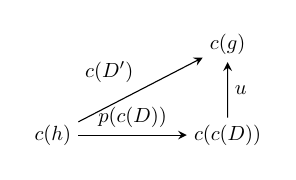
\begin{tikzpicture}[>=stealth,baseline=(current bounding box.center),scale=0.74,
    every node/.style={transform shape}]
    \node (Ch) at (0,0) {$c(h)$};
    \node (Cg) at (3.0,1.55) {$c(g)$};
    \node (CcD) at (3.0,0) {$c(c(D))$};
    \draw[->] (Ch) -- node[above left] {$c(D')$} (Cg);
    \draw[->] (CcD) -- node[right] {$u$} (Cg);
    \draw[->] (Ch) -- node[above] {$p(c(D))$} (CcD);
  \end{tikzpicture}
  \tag{3.2.12.5}
\end{equation}

\VerdierSemanticAnchor{ch1-3-2-12-conclusion}
が可換であることを確かめればよく、これは成分を明示すれば分かる。最後に、
(3.2.2) により、射 $q(f)$ の関手性 (3.2.2.2) から正方形
(3.2.12.2) が可換であることが従う。
\endgroup
